
\iffalse
\begin{figure}
    \centering
    \includegraphics[width=12cm]{../figures/blip_bbh_runs_two_panel_comparison.pdf}
    \caption{Glitch panel comparison}
    \label{fig:qscan_null}
\end{figure}
\fi
In section~\ref{sec:artefact} of this chapter, we mentioned that glitches can be problematic in two ways depending on their time of occurance. When occuring close to the merger, they can corrupt GW parameter measurement and when occuring in isolation, they could increase false alarms. A glitch overlapping with GW signal can be seen as a special case of glitch in isolation that is more harmful. 
\begin{table}[h!]
    \centering
    \renewcommand{\arraystretch}{1.2}
    \begin{tabular}{p{0.45\textwidth}|p{0.45\textwidth}}
    \toprule
    \textbf{LIGO-Virgo interferometers} & \textbf{Third generation interferometers} \\
    \midrule
    \begin{enumerate}[leftmargin=*, label=\arabic*.]
        \item Detection rate of $\mathcal{O}(1)$ signal per week
        \item A GW signal is in-band for $\mathcal{O}(1)$ second to $\mathcal{O}(1)$ minute. Nearly every segment of data contains only noise. 
        \item Glitch rate of $\mathcal{O}(1)$ per minute 
        \item \textit{Almost} all glitches occur in isolation due to smaller in-band duration of the signal and smaller detection rate of GW signals. 
        \item Almost all glitches are vetoed without incurring significant loss of GW signals. 
    \end{enumerate}
    &
    \begin{enumerate}[leftmargin=*, label=\arabic*.]
        \item Detection rate of $\mathcal{O}(1)$ signal per minute
        \item A GW signal is in-band for $\mathcal{O}(1)$ minute to $\mathcal{O}(1)$ hour. Nearly every segment of data is expected to contain a signal. 
        \item Glitch rate is unknown. Assume same as LIGO-Virgo interferometers
        \item \textit{Almost} all glitches will overlap with a GW signal due to larger in-band duration and larger detection rate. 
        \item Very few glitches may be vetoed without losing GW signals. 
    \end{enumerate}
    \\
    \bottomrule
    \end{tabular}
    \caption{Problem posed by glitches in LIGO-Virgo interferometers versus third-generation interferometers.}
    \label{tab:glitch_diff}
\end{table}


\section{Introducing \texttt{nijntje} algorithm}
\subsection{The null stream of the Einstein Telescope}
\subsection{Toy model}
\subsection{Absence of null stream: ET-2L comparison}
\section{Precision science measurement with speed}
\section{Caveats}
\begin{figure}
    \centering
    \includegraphics[width=10cm]{../figures/et2l_delta_glitch_overlap_glitch_master.pdf}
    \caption{Glitch overlap}
    \label{fig:glitch_overlap}
\end{figure}

\begin{figure}
    \centering
    \includegraphics[width=10cm]{../figures/newsnr_mismatch_comparison.pdf}
    \caption{Mismatch}
    \label{fig:mismatch}
\end{figure}

\begin{figure}
    \centering
    \includegraphics[width=16cm]{../figures/newsnr_fig_4.pdf}
    \caption{Mass Distance Sky}
    \label{fig:delta_zero}
\end{figure}

\begin{figure}
    \centering
    \includegraphics[width=10cm]{../figures/newsnr_rank_10_single_block_percentile_parameters_short.pdf}
    \caption{Confidence interval}
    \label{fig:trend_delta}
\end{figure}

\begin{figure}
    \centering
    \includegraphics[width=16cm]{../figures/assemble_nijntje.pdf}
    \caption{The blue box outlines the workflow of \texttt{nijntje} algorithm. \textit{Step 1}: Construct the null stream by summing the strain data from three interferometers. \textit{Step 2}: Using the null stream data and an RJMCMC method, perform an unmodelled reconstruction of the glitch timeseries. \textit{Step 3}: Find the glitch timeseries which corresponds to the median of the posterior samples and subtract it from $\mathrm{ET}_1$ frame. \textit{Step 4} (Optional): Perform parameter estimation using the cleaned data from $\mathrm{ET}_1$, and the existing data from $\mathrm{ET}_2$ and $\mathrm{ET}_3$ to verify the accuracy.}
    \label{fig:nijntje_chart}
\end{figure}

